\chapter{Getting started}

\section{An Introduction}
This template was created by Junjie Li, the primary contributor, and Manuel Liu Wang, the secondary contributor, both UB students majoring in computer science. It is not an official template from UB.

It can be an essay, thesis, report, or article. The template is for broad usage. Mathematical notation, matrix application, pictures, formulas, a range of word styles, and page size are all included.


\section{Tutorial}
Options \underline{[Option1, Option2, Option3, Option4, Option5, and Option6]} are listed in the first line. , those options regulate the template's fundamental layout: Option 1 modifies the page mode; Option 2 sets the font size; Option 3 establishes the page side; Option 4 applies the desired font style; Option 5 toggles the print/online version; and Option 6 activates the draft option.

On the other side, there is the optional zone, which you can omit if you choose. For instance, the first optional zone has the cover and the footer.


\section{Usage}

You can look at the chapter sections, beginning with section 2, to get a quick overview of how to use this template. All the chapters have usage examples.    




\chapter{My second Chapter}

\section{Images exemple}


\textbf{Example of an image:}
\begin{figure}[H]
    \centering
    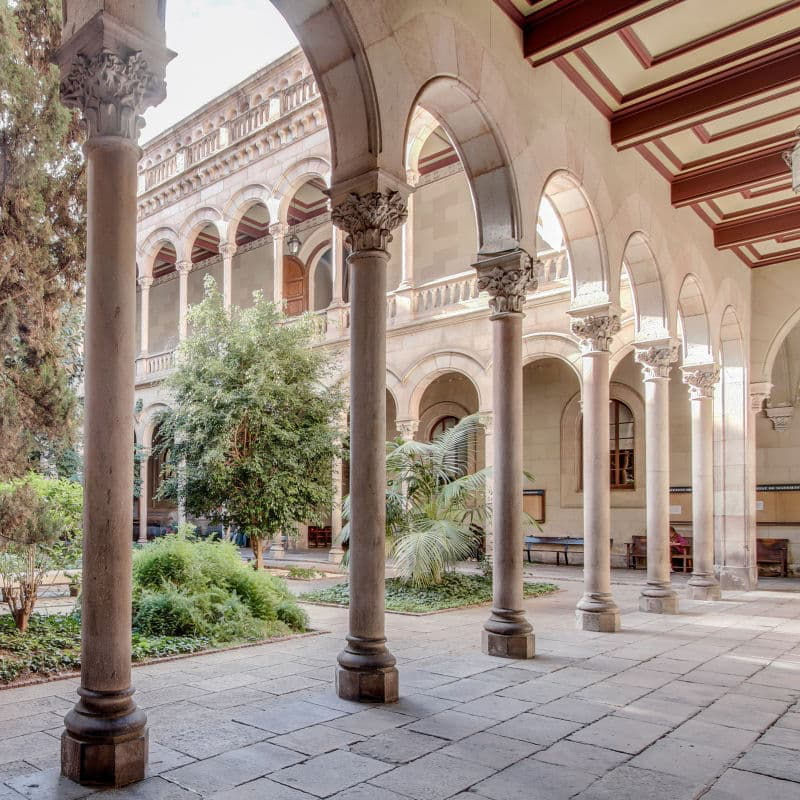
\includegraphics[width=6cm, height=4cm]{images/edifici-historic-universitat-de-barcelona.jpg}
    \caption{Image example}
    \label{fig:image_example}
\end{figure}

\textbf{Example of an image without caption:}
\begin{figure}[H]
    \centering
    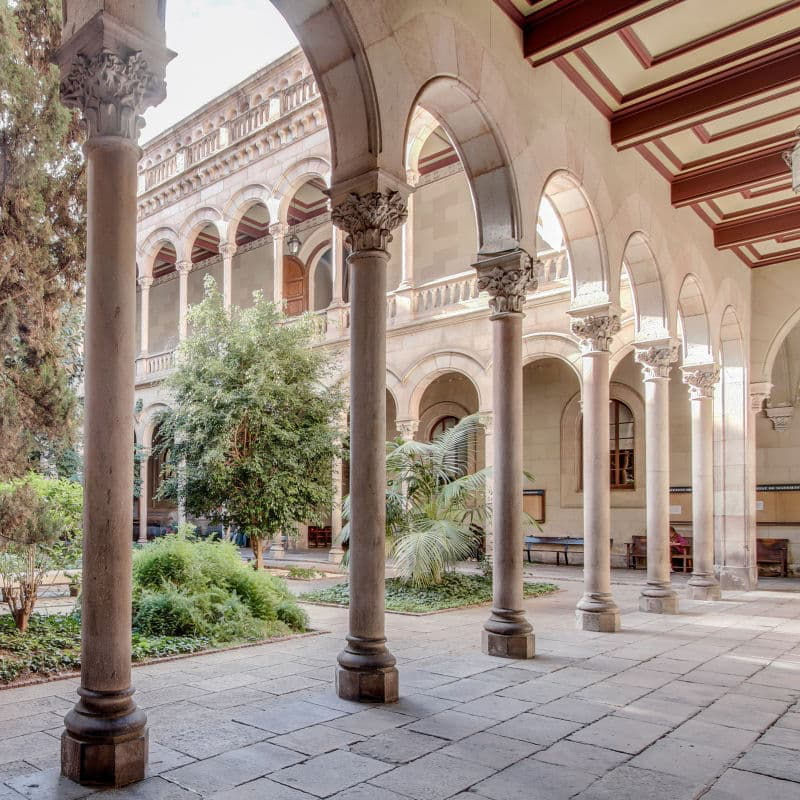
\includegraphics[width=6cm, height=4cm]{images/edifici-historic-universitat-de-barcelona.jpg}
    \label{fig:image_example_no_caption}
\end{figure}


\textbf{Example of two images:}
\begin{figure}[H]
    \centering
    \begin{minipage}[t]{0.48\textwidth}
        \centering
        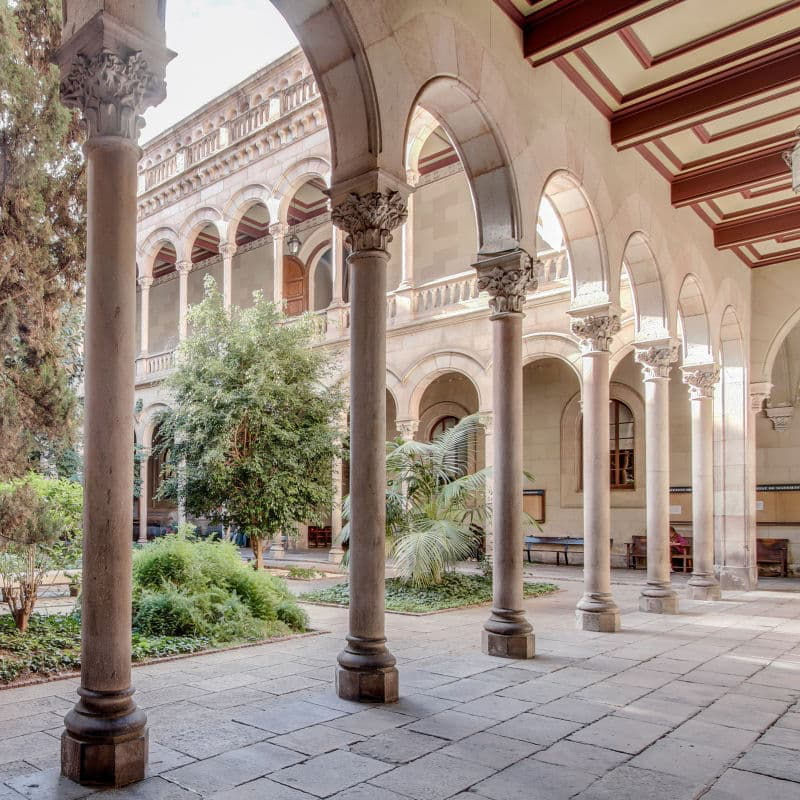
\includegraphics[width=6cm, height=4cm]{images/edifici-historic-universitat-de-barcelona.jpg}
        \caption{Image example2}
        \label{fig:image_example2}
    \end{minipage}
    \begin{minipage}[t]{0.48\textwidth}
        \centering
        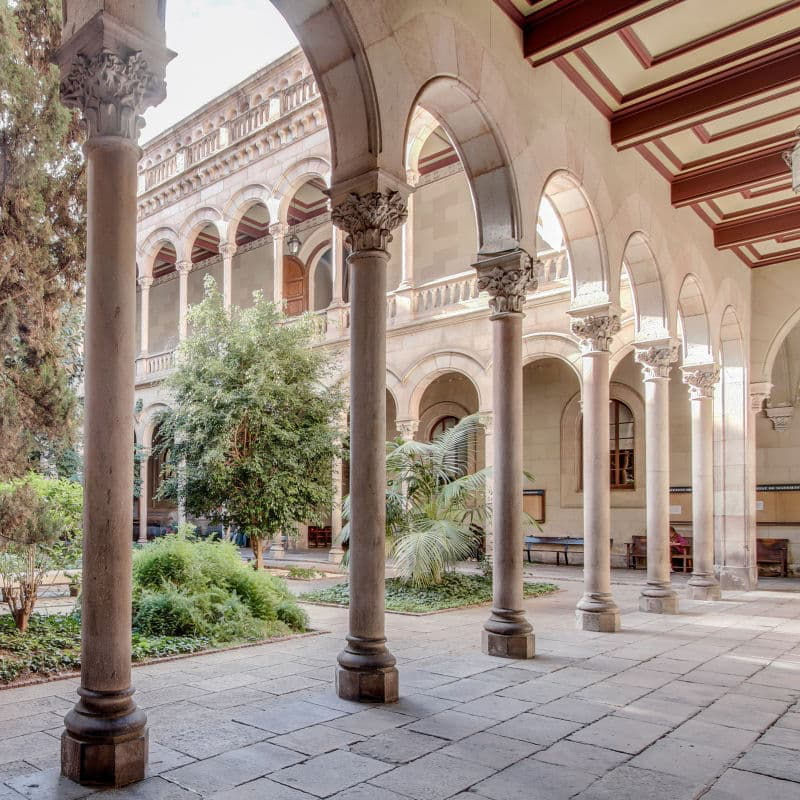
\includegraphics[width=6cm, height=4cm]{images/edifici-historic-universitat-de-barcelona.jpg}
        \caption{Image example3}
        \label{fig:image_example3}
    \end{minipage}
\end{figure}



\textbf{Example of two images with one caption:}
\begin{figure}[h]
  \centering
  \begin{minipage}{0.45\textwidth}
    \centering
    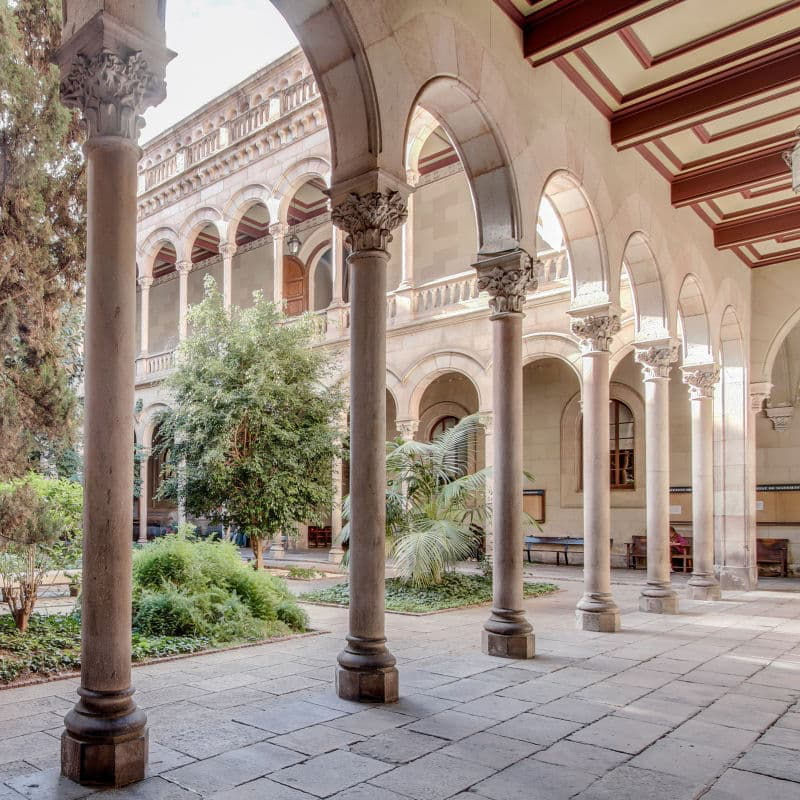
\includegraphics[width=6cm, height=4cm]{images/edifici-historic-universitat-de-barcelona.jpg}
  \end{minipage}
  \begin{minipage}{0.45\textwidth}
    \centering
    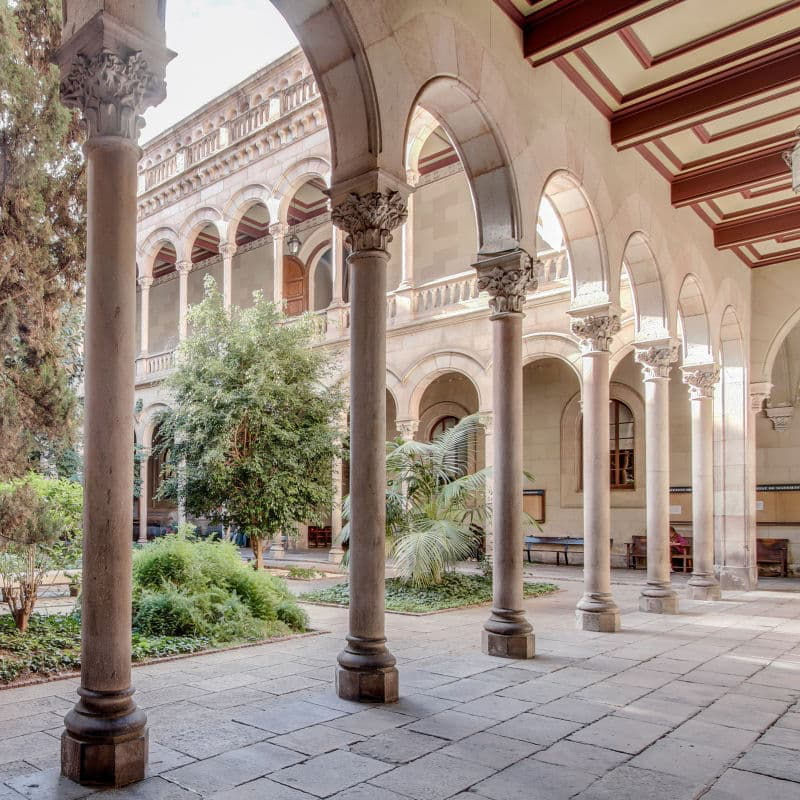
\includegraphics[width=6cm, height=4cm]{images/edifici-historic-universitat-de-barcelona.jpg}
  \end{minipage}
  \caption{Caption for both figures}
  \label{fig:two_images}
\end{figure}


\textbf{Example of the use of the label:} \\
As you can see in the Figure \ref{fig:two_images}, there are two pictures but only one caption, also it is in the page \pageref{fig:two_images}.


\textbf{Example of wrapping the text around the figure:}\\

\begin{wrapfigure}{r}{0.25\textwidth} %this figure will be at the right
    \centering
    
\includegraphics[width=0.25\textwidth]{preambles/static/ub_logo/ub_logo_3.png}
\end{wrapfigure}
The University of Barcelona (Catalan: Universitat de Barcelona, UB; Spanish: Universidad de Barcelona) is a public university located in the city of Barcelona, Catalonia, in Spain. With 63,000 students, it is one of the biggest universities in Spain. It is one of the oldest universities in both Catalonia and Spain, established in 1450.
It is considered one of the best universities in Spain. Overall, the UB has been ranked 1st in Spain in most of the 2022-2023 rankings and is located around the 50th place in Europe. 


\begin{wrapfigure}{l}{0.35\textwidth}
    \centering
    
\includegraphics[width=0.35\textwidth]{preambles/static/ub_logo/ub_logo_1.png}
\end{wrapfigure}
It has 106 departments and more than 5,000 full-time researchers, technicians and research assistants, most of whom work in the 243 research groups as recognized and supported by the Government of Catalonia. 

In 2010, the UB was awarded 175 national research grants and 17 European grants and participated in over 500 joint research projects with the business sector, generating an overall research income of 70 million euros. 

The work of these groups is overseen by the UB's research centres and institutes which collaborate with leading research institutions and networks in Spain and abroad. 

\let\clearpage\relax        %% This command prevents the list of figures to start in a new page
\listoffigures

\newpage




\newpage



\section{Math example}

Example math equation on the sentence:

The most famous equation in the world: $E^2 = (m_0c^2)^2 + (pc)^2$, which is 
known as the \textbf{energy-mass-momentum} relation as an in-line equation.


Example math equation on the squart:

\begin{equation}
P_{R_X} = P_{T_X} \cdot G_{T_X}  \cdot G_{R_X} \cdot \left( \frac{\lambda}{4\pi d} \right)^2  \cdot \eta
\end{equation}

\section{Table example}

\begin{table}[H]
\caption{A badly formatted table}
\centering
\label{table:bad_table}
\begin{tabular}{|l|c|c|c|c|}
\hline 
& \multicolumn{2}{c}{Species I} & \multicolumn{2}{c|}{Species II} \\ 
\hline
Dental measurement  & mean & SD  & mean & SD  \\ \hline 
\hline
I1MD & 6.23 & 0.91 & 5.2  & 0.7  \\
\hline 
I1LL & 7.48 & 0.56 & 8.7  & 0.71 \\
\hline 
I2MD & 3.99 & 0.63 & 4.22 & 0.54 \\
\hline 
I2LL & 6.81 & 0.02 & 6.66 & 0.01 \\
\hline 
CMD & 13.47 & 0.09 & 10.55 & 0.05 \\
\hline 
CBL & 11.88 & 0.05 & 13.11 & 0.04\\ 
\hline 
\end{tabular}
\end{table}



\begin{table}[H]
\caption{A nice looking table}
\centering
\label{table:nice_table}
\begin{tabular}{l c c c c}
\hline 
\multirow{2}{*}{Dental measurement} & \multicolumn{2}{c}{Species I} & \multicolumn{2}{c}{Species II} \\ 
\cline{2-5}
  & mean & SD  & mean & SD  \\ 
\hline
I1MD & 6.23 & 0.91 & 5.2  & 0.7  \\

I1LL & 7.48 & 0.56 & 8.7  & 0.71 \\

I2MD & 3.99 & 0.63 & 4.22 & 0.54 \\

I2LL & 6.81 & 0.02 & 6.66 & 0.01 \\

CMD & 13.47 & 0.09 & 10.55 & 0.05 \\

CBL & 11.88 & 0.05 & 13.11 & 0.04\\ 
\hline 
\end{tabular}
\end{table}


It high recommended to use {\url{https://www.tablesgenerator.com/#}} to generate easy table.




\chapter{My third chapter}

Write your conclusion here.






\chapter{Glossary tutorial}

 The \Gls{latex} typesetting markup language is specially suitable 
for documents that include \gls{maths}. Give



\chapter{bibliograp Tutorial}

Using you can display a bibliography divided into sections, depending on citation type. 
Let's cite! Einstein's journal paper \cite{einstein} and Dirac's book \cite{dirac} are physics-related items. 
Next, \textit{The \LaTeX\ Companion} book \cite{latexcompanion}, Donald Knuth's website \cite{knuthwebsite}, \textit{The Comprehensive Tex Archive Network} (CTAN) \cite{ctan} are \LaTeX-related items; but the others, Donald Knuth's items, \cite{knuth-fa,knuth-acp} are dedicated to programming.



\chapter{Exanple of Indices of terms}

In this example, several keywords\index{keywords} will be 
used which are important and deserve to appear in the 
Index\index{Index}.

Terms like generate\index{generate} and some\index{others} 
will also show up. Terms in the index can also be 
nested \index{Index!nested}